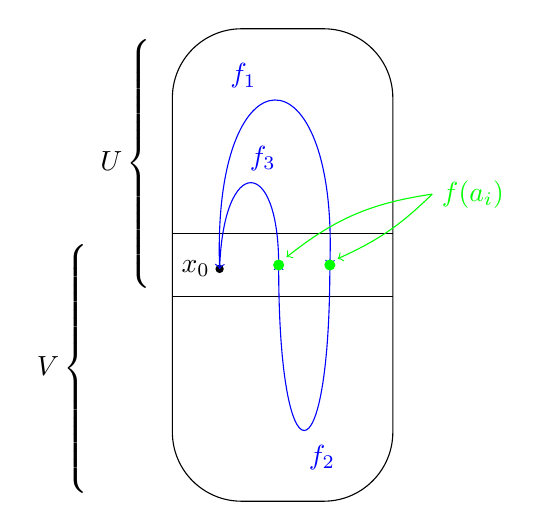
\begin{tikzpicture}
\draw[rounded corners=25pt] (-1.4,-3) rectangle (1.4,3);
\draw (-1.4,0.4) -- (1.4,0.4);
\draw (-1.4,-0.4) -- (1.4,-0.4);
\node[left] at (-1.5,1.3) {$U\left\{\rule{0pt}{1.7cm}\right.$};
\node[left] at (-2.3,-1.3) {$V\left\{\rule{0pt}{1.7cm}\right.$};
\fill (-0.8,-0.05) circle (1.5pt) node[left] {$x_0$};
\draw[blue, ->] (-0.8,-0.05) .. controls (-0.9,2.8) and (0.7,2.8) .. (0.6,0);
\draw[blue, ->] (0.6,0) .. controls (0.6,-2.8) and (-0.05,-2.8) .. (-0.05,0);
\draw[blue, ->] (-0.05,0) .. controls (-0.05,1.4) and (-0.75,1.4) .. (-0.8,-0.05);
\node[blue] at (-0.5,2.4) {$f_1$};
\node[blue] at (0.5,-2.45) {$f_2$};
\node[blue] at (-0.25,1.35) {$f_3$};
\fill[green] (0.6,0) circle (2pt);
\fill[green] (-0.05,0) circle (2pt);
\node[green, right] at (1.9,0.9) {$f(a_i)$};
\draw[green, ->] (1.9,0.9) to[bend left=10] (0.7,0.08);
\draw[green, ->] (1.9,0.9) to[bend right=15] (0.05,0.1);
\end{tikzpicture}
